\documentclass[a4paper,11pt,UTF8]{article}
\usepackage{ctex}
\usepackage{amsmath,amsthm,amssymb,amsfonts}
\usepackage{amsmath}
\usepackage[a4paper]{geometry}
\usepackage{graphicx}
\usepackage{microtype}
\usepackage{siunitx}
\usepackage{booktabs}
\usepackage[colorlinks=false, pdfborder={0 0 0}]{hyperref}
\usepackage{cleveref}
\usepackage{esint} 
\usepackage{graphicx}
\usepackage{ragged2e}
\usepackage{pifont}
\usepackage{extarrows}
\usepackage{mathptmx}
\usepackage{float}
\usepackage{caption}
\captionsetup[figure]{name={Figure}}
%opening
\title{Microelectronics Circuit Analysis and Design Homework(4th)}
\author{Yuejin Xie \quad U202210333}
\date{Sept 15th, 2023 }
\begin{document}
\maketitle
\noindent 2.14 The circuit in Figure P2.14 is a complementary output rectifier. If $v_s = 26
\sin [2\pi(60)t]$V, sketch the output waveforms $ v^+_o $ and $v^-_o $ versus time, assuming
$V_\gamma = 0.6$V for each diode.
\begin{figure}[H] 
	\centering 
	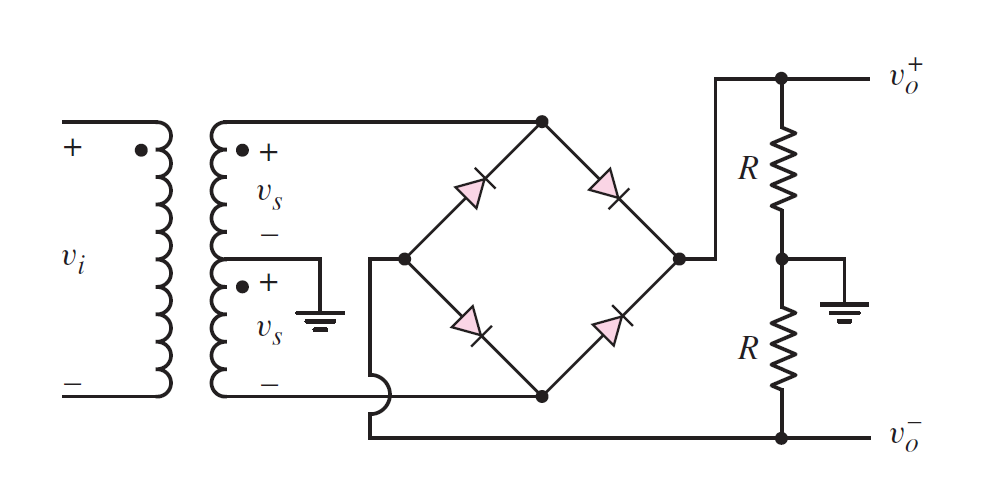
\includegraphics[scale=0.3]{MD2.14.png}
	\caption{Problem 2.14}
\end{figure}
\noindent Solution:\\
The four diodes from left to right and top to bottom are numbered A, B, C, and D respectively.\\
When $\displaystyle 0<t\leq\frac{T}2$, A, C are conducted and B, D aren't, so at this moment, $v^+_o=v_s-V_\gamma,v^+_o=-v_s+V_\gamma$ (conducted, if aren't conducted $v^+_o=v^-_o=0$)\\
When $\displaystyle\frac{T}2<t<T$, B, D are conducted and A, C aren't, so at this moment, the answer is the same as $\displaystyle 0<t\leq\frac{T}2$\\
We provide results using Multisim:
\begin{figure}[H] 
	\centering
	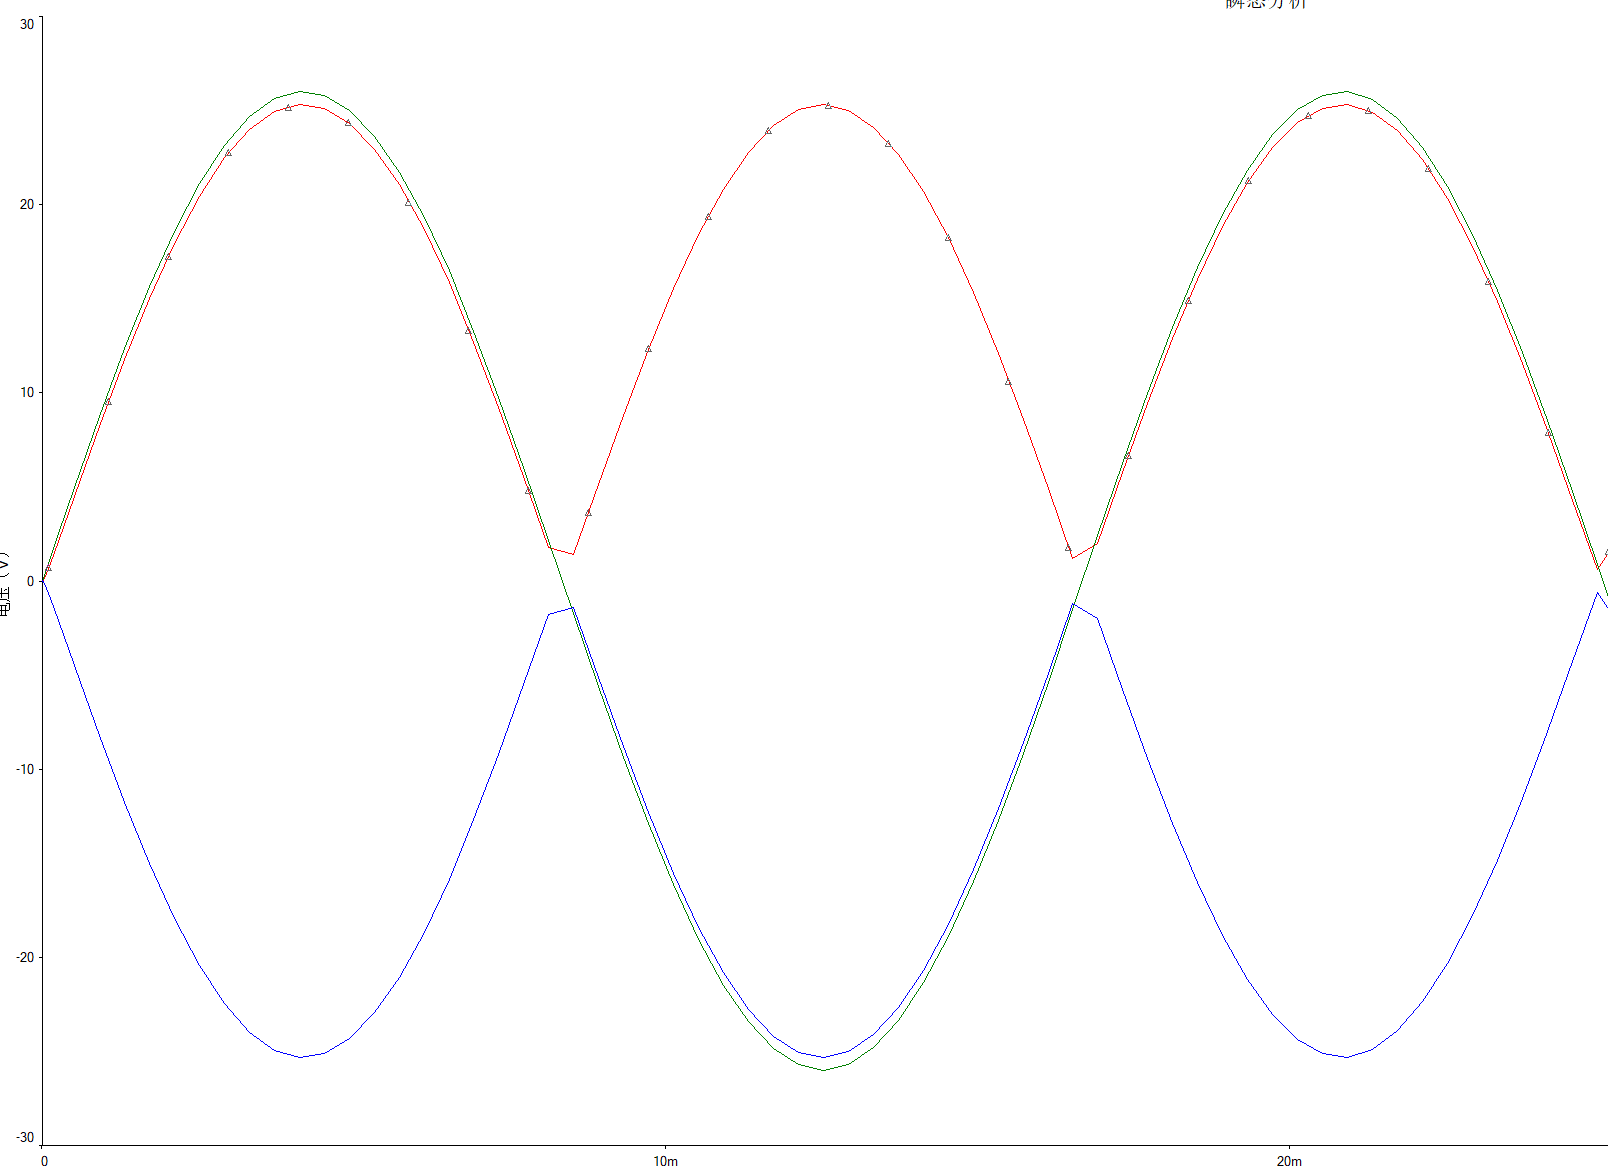
\includegraphics[scale=0.3]{MD2.14_1}
\end{figure}
\noindent2.45 In the circuit in Figure P2.45 the diodes have the same piecewise linear parameters
as described in Problem 2.44($V_\gamma = 0.6$V and $r_f = 0$). Calculate the output voltage $V_O$ and
the currents $I_{D1}$, $I_{D2}$, and $I$ for the following input conditions: (a) $V1 =
V_2 = 10 $V; (b) $V_1 = 10$V, $V_2 = 0$; (c) $V_1 = 10 $V, $V_2 = 5$V; and (d)
$V_1 = V_2 = 0$.
\begin{figure}[H] 
	\centering 
	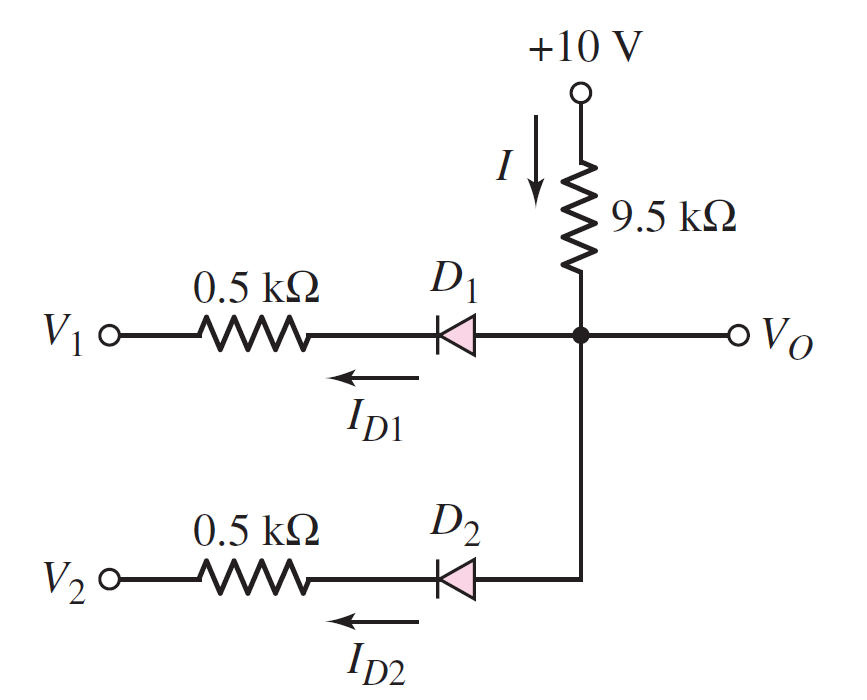
\includegraphics[scale=0.25]{MD2.45.png}
	\caption{Problem 2.45}
\end{figure}
\noindent Solution:\\
(a)Owing to $V_s=V_1=V_2=10V$, $D_1$ and $D_2$ can't be conducted, so $V_O=V_s=10$V, $I = I_{D1} = I_{D2} = 0$, \\
(b)In this case,  $D_2$ is conducted but $D_1$ not, so $\displaystyle I_{D1}= 0, I_{D2}=I=\frac{V_s-V_\gamma}{R_1+R_2}=0.94\text{mA}.\\ V_O=V_s-IR_1=1.07$V\\
(c)In this case,  $D_2$ is conducted but $D_1$ not, so $\displaystyle I_{D1}= 0, I_{D2}=I=\frac{V_s-V_\gamma}{R_1+R_2}=0.44\text{mA}.\\ V_O=V_s-IR_1=5.82$V\\
(d)In this case,  both $D_1$ and $D_2$ are conducted, we have equation:
$$\begin{cases}
	\displaystyle I=\frac{V_s-V_O}{R_1}\\
	\displaystyle I=I_{D1}+I_{D2}\\
	\displaystyle I_{D1}=I_{D2}=\frac{V_O-V_\gamma}{R_1}
\end{cases}\Rightarrow
\begin{cases}
	I = 0.964 \text{mA}\\
	V_O = 0.842 \text{V}\\
	I_{D1} = I_{D2} = 0.482 \text{mA}
\end{cases}
$$
\noindent2.58 (a) Each diode in the circuit in Figure P2.58 has piecewise linear parameters
of $V_\gamma = 0 $ and $r_f = 0$. Plot $v_O$ versus $v_I$ for $0 \leq v_I \leq 30$V. Indicate the
breakpoints and give the state of each diode in the various regions of the plot.
(b) Compare the results of part (a) with a computer simulation analysis.
\begin{figure}[H] 
	\centering 
	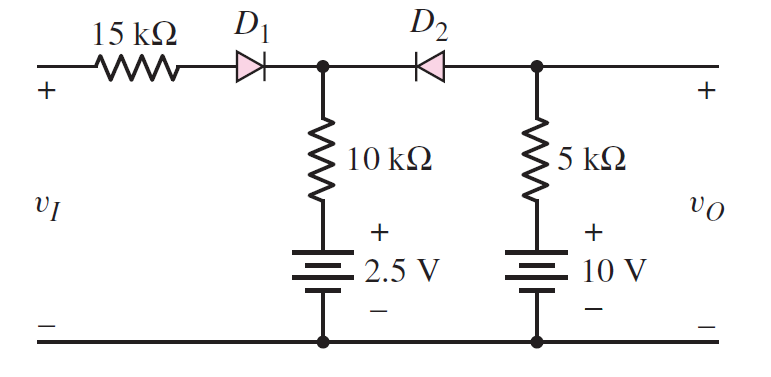
\includegraphics[scale=0.35]{MD2.58.png}
	\caption{Problem 2.58}
\end{figure}
\noindent Solution:\\
(a)When $0<V_I<2.5$V, $D_1$ and $D_2$ aren't conducted, so $V_O=10$V\\
When $2.5$V$\leq V_I<21.25$V, $D_1$ is conducted but $D_2$ not, so $V_O=10$V\\
When $21.25$V$\leq V_I<30$V, $D_1$ and $D_2$ are conducted, we have equation:
$$\begin{aligned}
	&\frac{V_I-V_O}{15k\Omega}=\frac{V_O-2.5}{10k\Omega}+\frac{V_O-10}{5k\Omega}\\
	\Rightarrow &V_O=\frac{2}{11}V_I+\frac{135}{22}
\end{aligned}
$$
\begin{figure}[H] 
	\centering 
	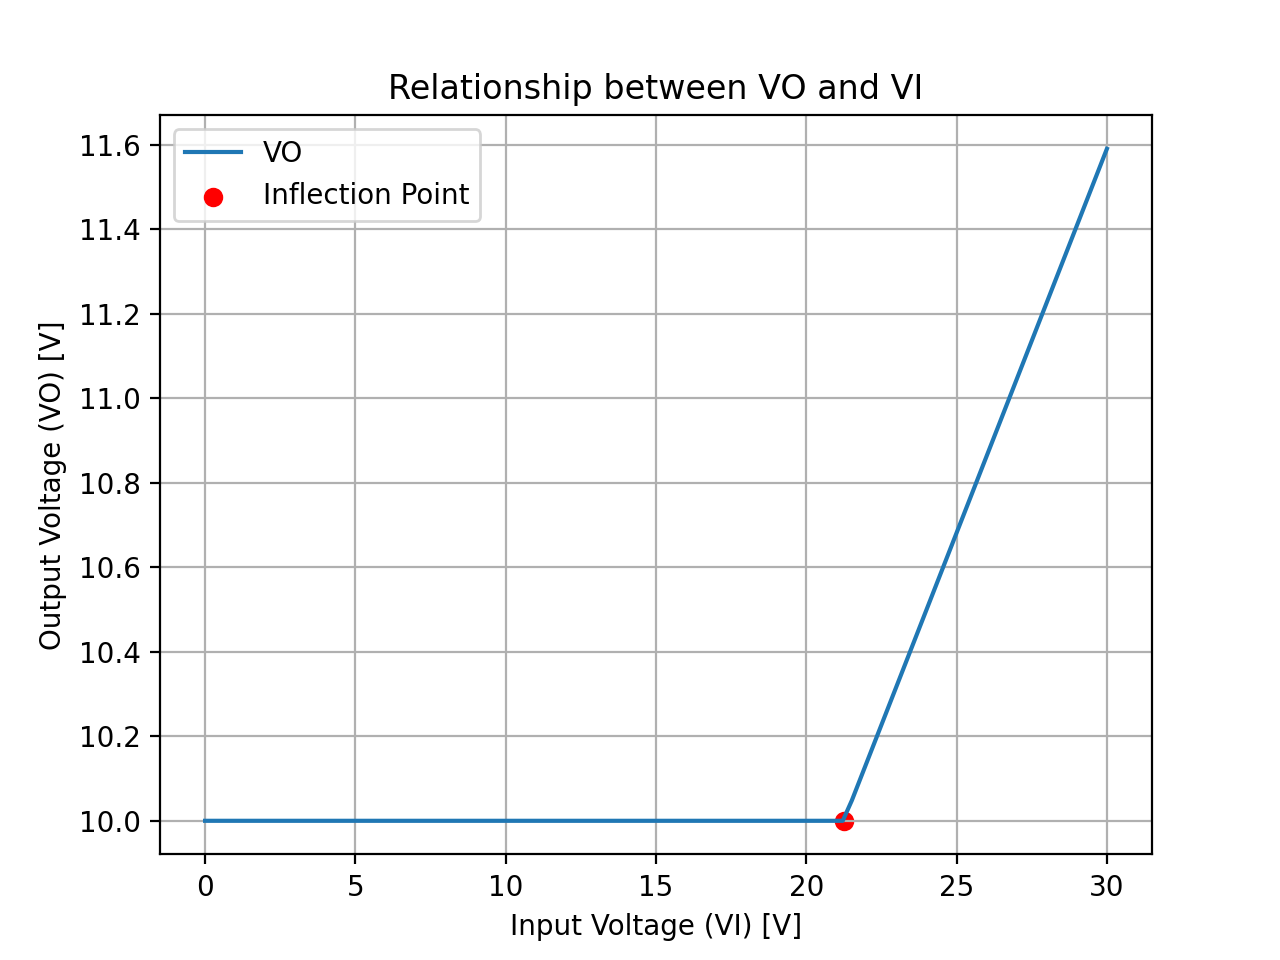
\includegraphics[scale=0.25]{MD2.58_2}
	\caption{$v_O$ versus $v_I$ for $0 \leq v_I \leq 30$V}
\end{figure}
(b)
\begin{figure}[H] 
	\centering 
	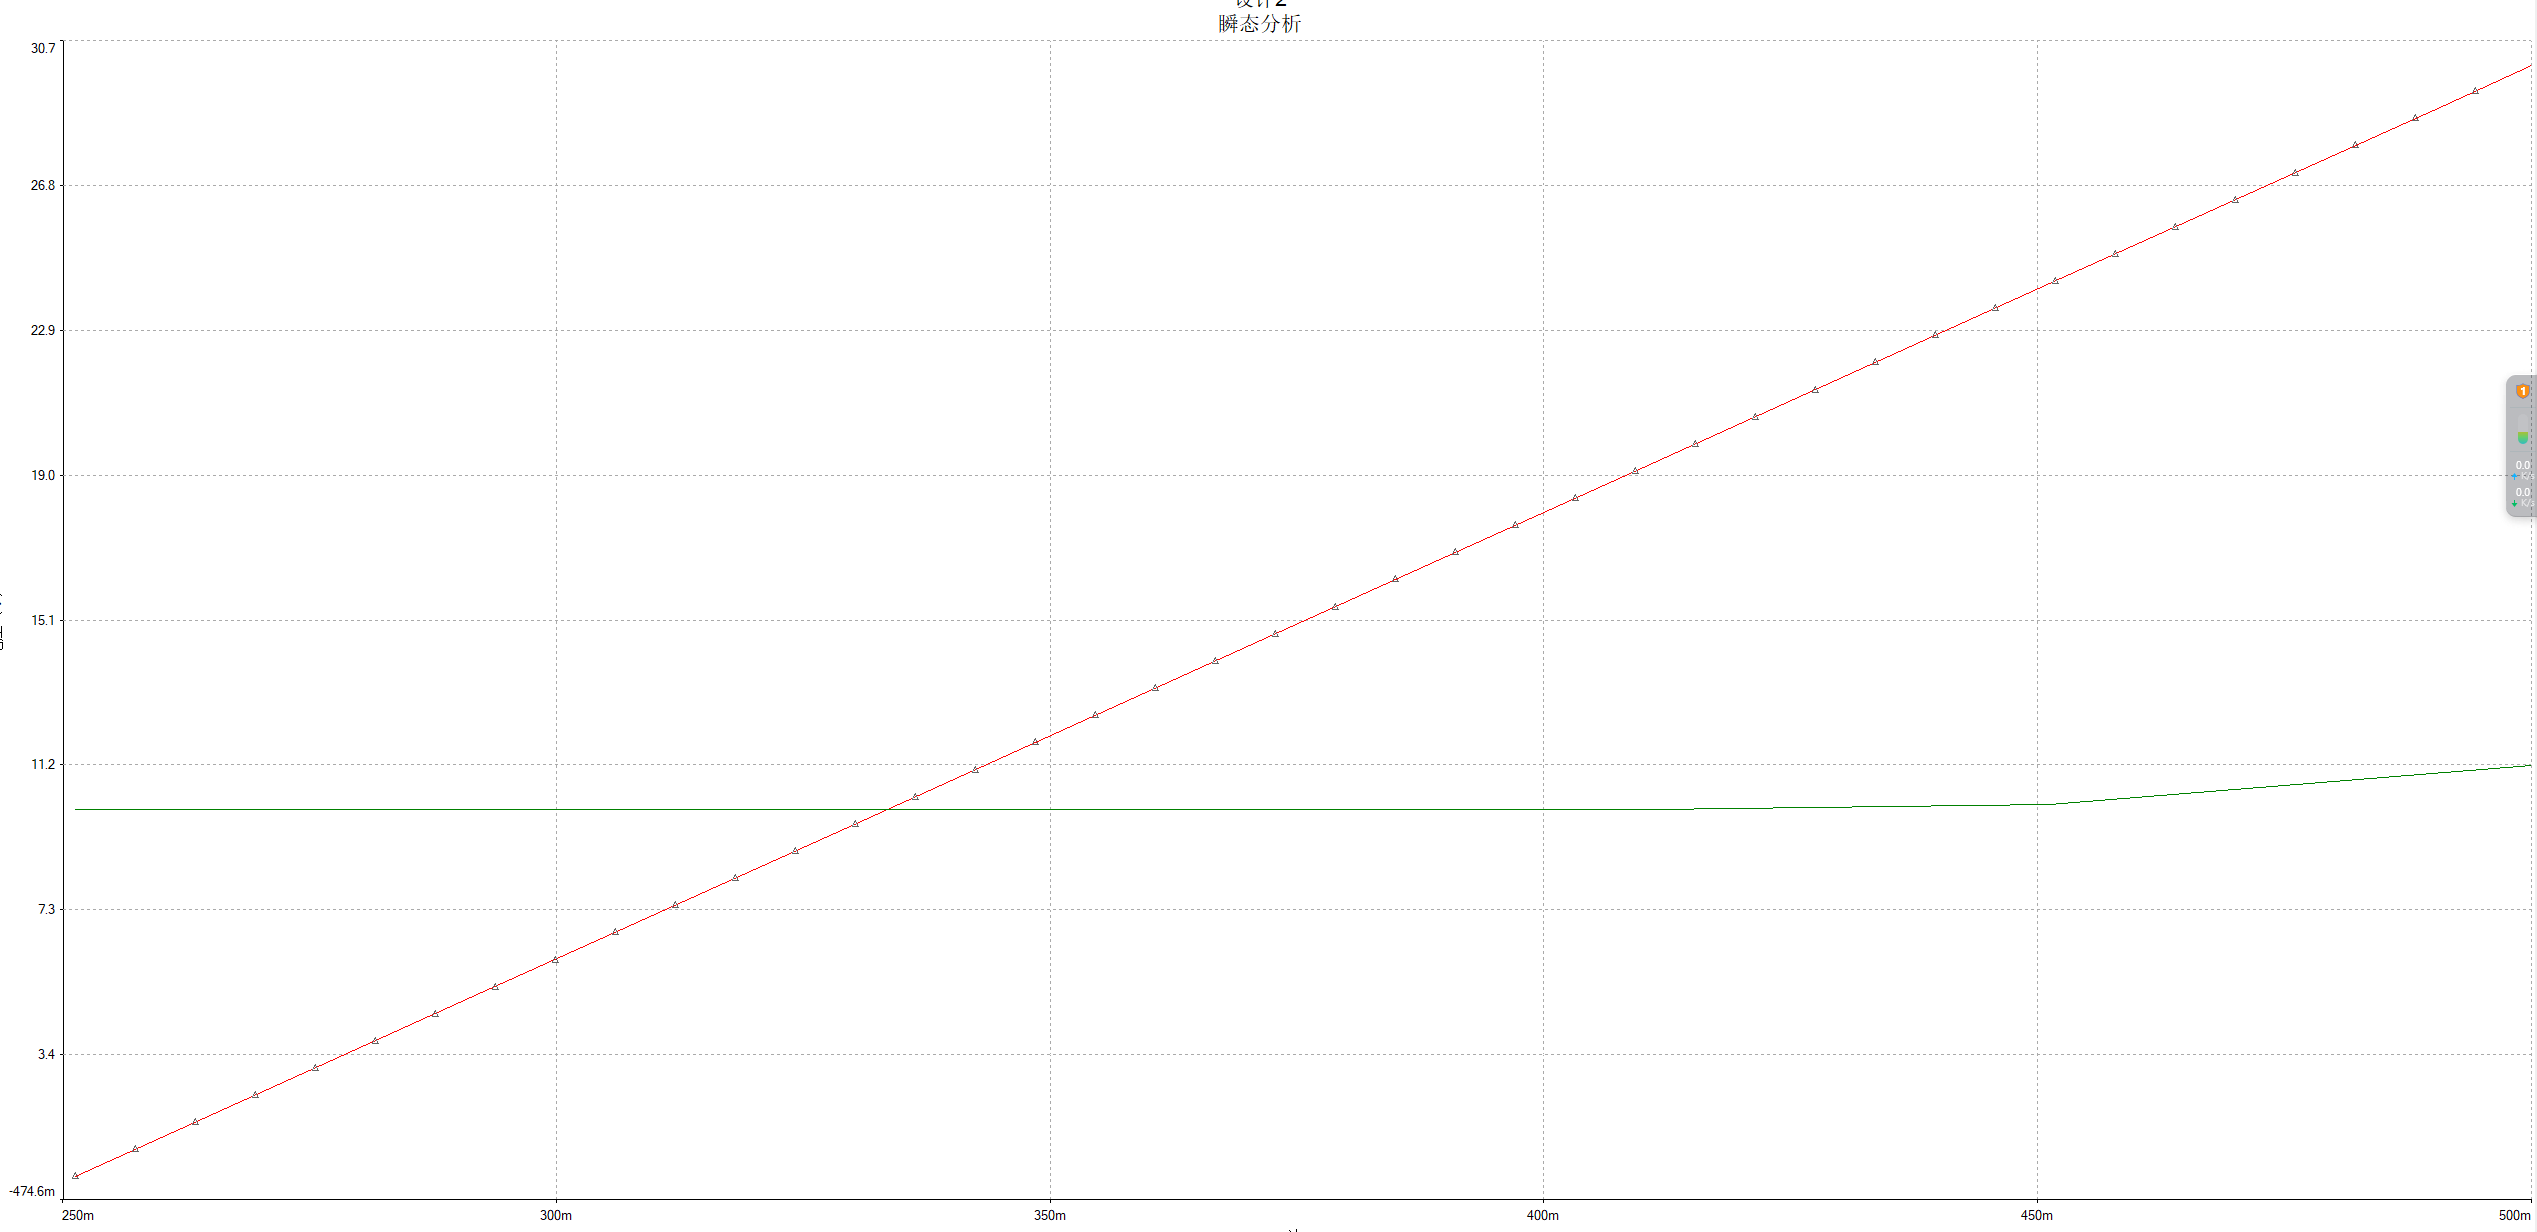
\includegraphics[scale=0.25]{MD2.58_1}
	\caption{Multisim AAAnalysis}
\end{figure}
\end{document}